\documentclass[final]{fhnwreport}       %[mode] = draft or final
                                        %{class} = fhnwreport, article, 
                                        %          report, book, beamer, standalone
%%---Main Packages-----------------------------------------------------------------------
\usepackage[english, ngerman]{babel}	%Mul­tilin­gual sup­port for LaTeX
\usepackage[T1]{fontenc}				%Stan­dard pack­age for se­lect­ing font en­cod­ings
\usepackage[utf8]{inputenc}				%Ac­cept dif­fer­ent in­put en­cod­ings
\usepackage{lmodern}                    %The newer Font-Set
\usepackage{textcomp}					%LaTeX sup­port for the Text Com­pan­ion fonts
\usepackage{caption}					%Customising captions in floating environments
\usepackage{graphicx} 					%En­hanced sup­port for graph­ics
\usepackage{float}						%Im­proved in­ter­face for float­ing ob­jects
\usepackage{ifdraft}                    %Let you check if the doc is in draft mode

%%---Useful Packages---------------------------------------------------------------------
\usepackage{color}						%Colour control for LaTeX documents
\usepackage[pdftex,dvipsnames]{xcolor}  %Driver-in­de­pen­dent color ex­ten­sions for LaTeX
\usepackage{csquotes}                   %Simpler quoting with \enquote{}
\usepackage{siunitx} 					%A com­pre­hen­sive (SI) units pack­age
\usepackage{listings}					%Type­set source code list­ings us­ing LaTeX
\usepackage[bottom]{footmisc}			%A range of foot­note op­tions
\usepackage{footnote}					%Im­prove on LaTeX's foot­note han­dling
\usepackage{verbatim}					%Reim­ple­men­ta­tion of and ex­ten­sions to LaTeX ver­ba­tim
\usepackage[textsize=footnotesize]{todonotes} %Mark­ing things to do in a LaTeX doc­u­ment
\usepackage{titling}					%Control over the typesetting of the \maketitle command

%%---Tikz Packages-----------------------------------------------------------------------
\usepackage{standalone}
\usepackage{tikz}
\usepackage{circuitikz}
\usetikzlibrary{arrows}
\usetikzlibrary{calc}
\usetikzlibrary{intersections}

%%---Math Packages-----------------------------------------------------------------------
\usepackage{amsmath}					%AMS math­e­mat­i­cal fa­cil­i­ties for LaTeX
\usepackage{amssymb}					%Type­set­ting symbols (AMS style)
%\usepackage{amstext}
%\usepackage{amsfonts}
%\usepackage{breqn}
\usepackage{array}						%Ex­tend­ing the ar­ray and tab­u­lar en­vi­ron­ments
\usepackage{amsthm}					%Type­set­ting the­o­rems (AMS style)

%%---Table Packages----------------------------------------------------------------------
\usepackage{tabularx}					%Tab­u­lars with ad­justable-width columns
%\usepackage{longtable}
\usepackage{multirow}					%Create tab­u­lar cells span­ning mul­ti­ple rows
\usepackage{multicol}					%In­ter­mix sin­gle and mul­ti­ple columns

%%---PDF / Figure Packages---------------------------------------------------------------
\usepackage{pdfpages}					%In­clude PDF doc­u­ments in LaTeX
\usepackage{pdflscape}					%Make land­scape pages dis­play as land­scape
\usepackage{subfig}					    %Fig­ures di­vided into sub­fig­ures

%%---Other Packages----------------------------------------------------------------------
%\usepackage{xargs}                     %De­fine com­mands with many op­tional ar­gu­ments


%%---Bibliography------------------------------------------------------------------------
\usepackage[style=ieee,urldate=comp,backend=biber,language=english]{biblatex}
\addbibresource{literature/Kryg_Artikel.bib}

\DefineBibliographyStrings{ngerman}{
	url         = [Online]\addspace Available: ,
	urlseen		= {Abrufdatum}
}

%%---Main Settings-----------------------------------------------------------------------
\graphicspath{{./graphics/}}			%Defines the graphicspath
\geometry{twoside=false}				    %twoside=false disables the "bookstyle"
\setlength{\marginparwidth}{2cm}
\overfullrule=5em						%Creates a black rule if text goes over the margins => debugging




%%---User Definitions--------------------------------------------------------------------
%%Tabel-Definitions: (requires \usepackage{tabularx})
\newcolumntype{L}[1]{>{\raggedright\arraybackslash}p{#1}}    %column-width and alignment
\newcolumntype{C}[1]{>{\centering\arraybackslash}p{#1}}
\newcolumntype{R}[1]{>{\raggedleft\arraybackslash}p{#1}}

%%---Optional Package Settings-----------------------------------------------------------
%Listings-Settings: (requires \usepackage{listings}) => Example with Matlab Code
%\lstset{language=Matlab,%
%    basicstyle=\footnotesize\ttfamily,
%    breaklines=false,%
%    morekeywords={switch, case, otherwise},
%    keywordstyle=\color{Blue},%
%    tabsize=2,
%    %morekeywords=[2]{1}, keywordstyle=[2]{\color{black}},
%    identifierstyle=\color{Black},%
%    stringstyle=\color{Purple},
%    commentstyle=\color{Green},%
%    showstringspaces=false,%without this there will be a symbol in the places where there is a space
%    numbers=left,%
%    numberstyle={\tiny \color{black}},% size of the numbers
%    numbersep=9pt, % this defines how far the numbers are from the text
%    %emph=[1]{word1, word2,...},emphstyle=[1]\color{red}
%}							

% Eingefügt für C-Code Style
\renewcommand\lstlistingname{Codeausschnitt}
\lstset{language=C,
	basicstyle=\ttfamily,
	keywordstyle=\color{blue}\ttfamily,
	stringstyle=\color{red}\ttfamily,
	commentstyle=\color{green!70}\ttfamily,
	morecomment=[l][\color{magenta}]{\#}
}

%Hurenkinder und Schusterjungen verhindern (kein Scherz, Google es)
\clubpenalty10000
\widowpenalty10000
\displaywidowpenalty=10000	



%Titel mit Mathematik immer fett drucken
\usepackage{sectsty}
\allsectionsfont{\boldmath}




			                %loads all packages, definitions and settings											
\title{Essay Patent Palata}  		        %Project Title
%\author{Team 1}      				    %Document Type => Technical Report, ...
%\date{\today}          				%Place and Date

\begin{document}

%%---TITLEPAGE---------------------------------------------------------------------------------
\thispagestyle{empty}
%	\ohead{\includegraphics[scale=0.5]{Bilder/Logo_FHNW.jpg}}
	\begin{figure}
		 \vspace*{-\topskip}\vspace*{-\headsep}
		
\includegraphics[scale=1]{graphics/fhnw_ht_logo_de.pdf}
	\end{figure}

	
	\begin{center}
		\vspace*{2cm}
		{\huge{\textbf{\thetitle}}}\\
		\vspace*{0.5cm}
		
		 
		\Large{Windisch, \today}
		
		\vspace*{-1cm}						    %compensates the space after the date line.
		\vfill
		\begin{figure}[H]
		\centering
		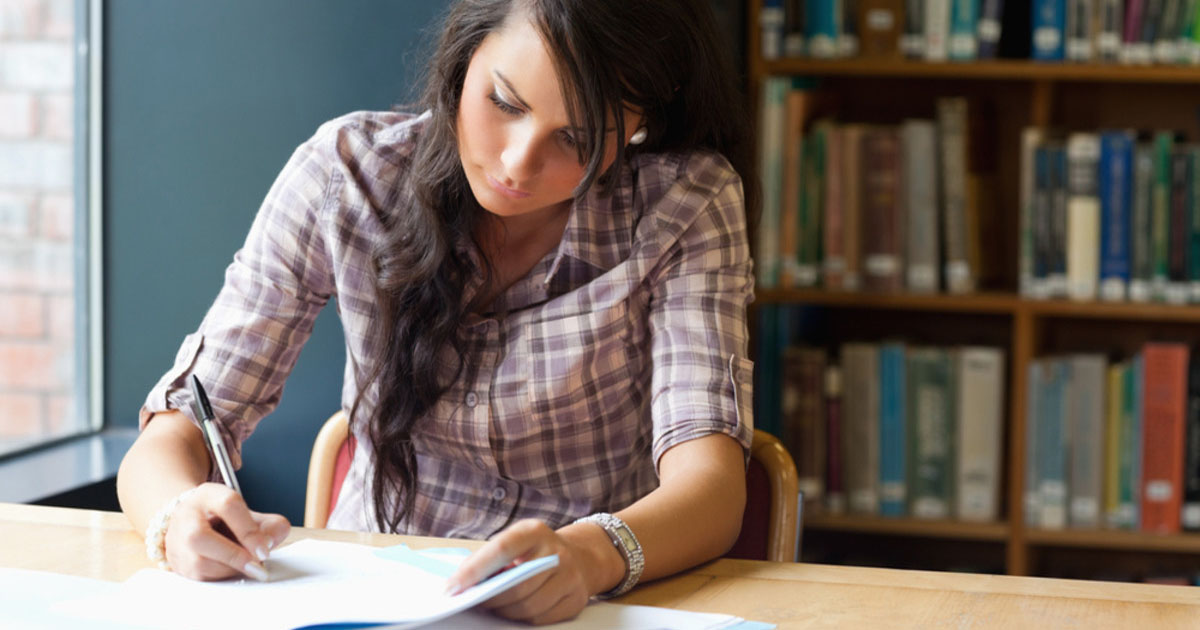
\includegraphics[width=1\textwidth]{Titelbild.png}
		%\cite{thirah_vorhangeschloss-schlussel-computer-icons_nodate}
		%\raggedleft
		\end{figure}
		
	
		\vfill
		
		\begin{normalsize}
			{
			\renewcommand\arraystretch{2}
			\begin{tabular}{>{\bf}p{4cm} l}
			Autoren   		           & Kim Schenk, Robin Aebi und	Gabriel Nussbaumer\\
			Dozent                 &    Tony Keller\\
			Modul		               &    Produktentwicklung und Innovation in der Elektrotechnik\\
			Hochschule                 &    Hochschule für Technik - FHNW\\
			Studiengang                &    Elektro- und Informationstechnik\\
%			Version                    &    1.0 %Normally not used!
			\end{tabular}
			}
		\end{normalsize}
	\end{center}
\clearpage
			
%%---ABSTRACT----------------------------------------------------------------------------
%\selectlanguage{english}				%ngerman or english
%\thispagestyle{empty}
%\include{sections/abstract}


%%---TABLE OF CONTENTS-------------------------------------------------------------------
\pagenumbering{Roman}		
\selectlanguage{ngerman}				%ngerman or english
\tableofcontents
\clearpage

%%---TEXT--------------------------------------------------------------------------------
\pagenumbering{arabic}

\clearpage
\section{Einleitung}\label{sec:Einleitung}
In dieser Bericht wird ein Essay über das Thema xxx erarbeitet. Der Bericht wird benotet und zählt als Abschlussarbeit für das Fach Produktentwicklung und Innovation in der Elektrotechnik, somit werden neben dem Essay, welches Zeit limitiert erarbeitet wird, noch zwei Innovationsmethoden beschrieben.\\
\newpage








%\clearpage
\section{Innovationsmethoden und Innovationsprozesse}


Ein Innovationsprozesses wird definiert durch die Umsetzung von bestehenden und/oder neuen Erkenntnissen in wirtschaftstaugliche Problemlösungen. Bei den Lösungen handelt es sich meist um ein Produkt oder Dienstleistung, welches oder welche auf dem Markt angeboten wird. Der Erfolg der Lösung hängt jedoch davon ab, ob sie erwartungsgemäss vom Markt aufgenommen wird oder nicht. Der Prozess sollte deshalb nicht nur technisch organisiert werden, sondern muss als interdisziplinären Prozess angesehen werden, welcher alle Unternehmensbereiche darin integriert.

Im Falle eines neuen Produktes, wird Marktforschung betrieben, welche eine Grundlage bietet für das Marketing und die Bedürfnisermittlung an das Endprodukt. Die Forschung- und Entwicklung entwickelt dann gemäss den ermittelten Bedürfnissen das Produkt an sich. Sobald das Produkt auf dem Markt eingeführt wurde, ist der Innovationsprozess bei diesem Beispiel zu Ende.\footnote{Source: https://wirtschaftslexikon.gabler.de/definition/innovationsprozess-41599}



\textbf{« Innovation braucht Methoden »}

Ob es darum geht, Ideen zu finden, ein Problem zu lösen oder zu recherchieren, es kommen jeweils verschiedene Methoden in Frage, um ans Ziel zu kommen. Die kommenden Grafiken sollen dies verdeutlichen. In jedem Arbeitsschritt gibt es eine ausgewählte Gruppe von Menschen, welche diverse Kreativitätstechniken anwenden können (Abb. \ref{fig:Grafik1}\footnote{Source: https://www.lead-innovation.com/hs-fs/hubfs/Vanadyl \%20Seiten/Innovationsprozess/Projektgrafik.\%20Innovationsprozess.jpeg?width=860\& name=Projektgrafik.\%20Innovationsprozess.jpeg}). Diese helfen, dass die Beteiligten für ihren Bereich das Optimum aus beispielsweise Erfahrung oder Kreativität zu Tage führen können. Die gewonnenen Erfahrungen werden jeweils von einer Person verarbeitet und für den nächsten Schritt aufbereitet.

\begin{figure}[h!]
	\centering
	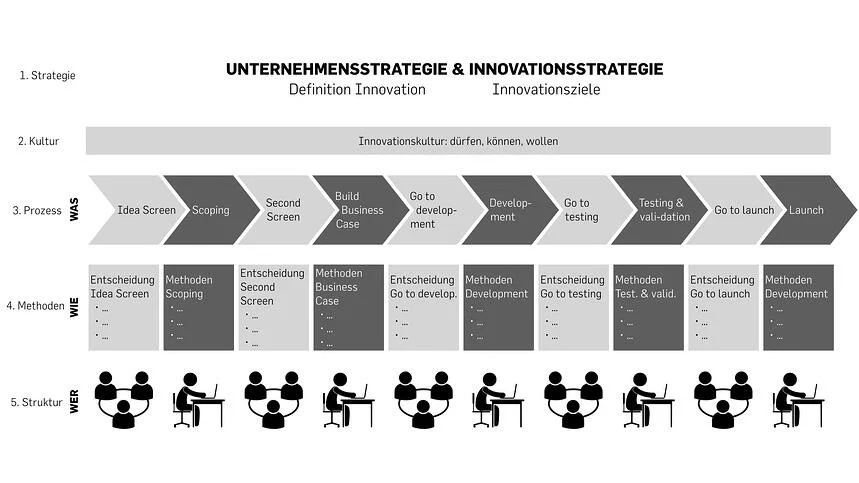
\includegraphics[width=\textwidth]{graphics/Grafik1}
	\caption{Prozessorganisation in einem Betrieb. Ersichtlich, dass während des Innovationsprozesses in verschiedenen Bereichen Methoden angewendet werden. Nach Anwenden der Kreativitätsmethoden werden die gewonnenen Daten jeweils ausgewertet und aufbereitet.}
	\label{fig:Grafik1}
\end{figure} 

Im «Fuzzy Frontend» (Abb. \ref{fig:Grafik2}\footnote{Source: https://www.lead-innovation.com/hs-fs/hubfs/Blogs/Innovationsprozess/Bildschirmfoto\%202017-07-17\%20um\%2016.13.11.png?width=750\& name=Bildschirmfoto\%202017-07-17\%20um\%2016.13.11.png}) ist ersichtlich, dass zwischen Ideenfindung und Konzeptphase die Ideen ständig ausgearbeitet und verbessert werden. Speziell in diesem Bereich ist Kreativität und Innovation von zentraler Bedeutung aber auch die Ideenselektrion spielt eine grosse Rolle. Im weiteren Verlauf des Prozesses sind andere Personen an anderen Prozessen beteiligt, diese sind eher Straight-forward und basieren grösstenteils auf betriebsinternen Erfahrungen. Im Vergleich zum ''Fuzzy Frontend'' arbeiten hier mehr spezialisierte Leute. Dementsprechend ist auch die Breite der Erfahrungsermittlung kleiner.

\begin{figure}[h!]
	\centering
	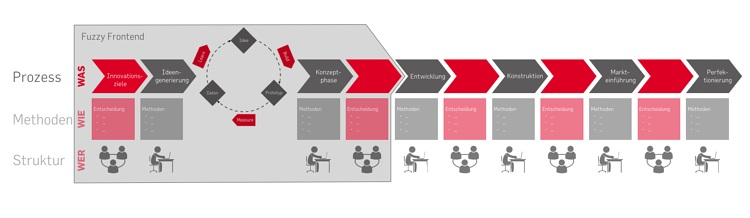
\includegraphics[width=\textwidth]{graphics/Grafik2}
	\caption{Prozesskette während dem Innovationsprozess. Erkennbar das erwähnte ''Fuzzy Frontend'' und die darauf folgenden Prozesse.}
	\label{fig:Grafik2}
\end{figure} 

Beispiel: Die Herstellung einer neuen TV-Geräteserie, die auf den Markt kommen soll. Die Ideenfindung und Konzeption des Gerätes bedarf im Anfangsprozess innovative Kreativitätsmethoden, um Kunden und Lieferanten während dem Vertrieb des Produktes zufrieden stellen zu können und gleichzeitig den betriebsinternen Kapazitäten gerecht zu werden. Ab der Entwicklung sind eher problemlösende Kreativitätsmethoden gefragt. Sobald das Produkt auf dem Markt ist, zeigt sich, ob der Innovationsprozess erfolgreich war.

Es wurde bereits erwähnt, dass ein Innovationsprozess als interdisziplinärer Prozess angesehen werden muss. Je nach Innovationsmethode sind demnach verschiedene Menschen aus verschiedenen Bereichen gefragt. Bei der Entwicklung eines Produktes sind alle Mitarbeiter miteinzubeziehen, von der Putzfrau über die Sekretärin, Ingenieure bishin zum CEO. Jeder sieht das Produkt von einer anderen Seite, worudrch sich ein allgemeineres Bild erstellen lässt. Hier wäre eine 6-3-5 Methode sinnvoll, welche zusätzlich erlaubt die Meinung eines jeden Beteiligten gleich zu gewichten. Geht es darum ein spezifisches technisches Problem zu lösen, sind die Ingenieure gefragt, bei ökonomischen Fragen die Wirtschaftler. Hier wäre eine Brainstorming Methode eher sinnvoll, welche es ermöglicht die zusammenhänge aufzuzeigen und jedem Beteiligten eine sofortige Reaktion zu geben.

Während der Innovationsprozesses gibt es also verschiedene Innovationsmethoden, um das gewünschte Ziel zu erreichen. Eine Innovationsmethode kann aus verschiedenen Kreativitätsmethoden bestehen, die beispielsweise aus Ideenfindung (z.B Brainstorming, 6-3-5) und Ideenselektion (z.B Markttests, Gewichtung, Studien). Im Folgenden werden zwei Kreativitätsmethoden beschrieben, welche in einem Innovationsprozess zur Ideenfindung angewendet werden können.

\newpage

\subsection{6-3-5 Methode}\label{subsec:635Methode}
Die 6-3-5 Methode ist eine Kreativitätstechnik zur Ideenfindung. Optimalerweise wird sie in einem Team mit 6 Personen angewendet. Es können Vorideen entstehen, wie auch gezielte Ideeanareicherung entwickelt werden.
\subsubsection{Vorgehensweise}
\begin{enumerate}

\item In einem ersten Schritt werden jedem Teilenehmer Blätter in Papierform verteilt. Auf den Blättern hat es eine Tabelle mit 3 Spalten und die zuvor definierte Frage. Aus praktischen Gründen sollten sich die Teilnehmer am selben Tisch befinden.
\item Im zweiten Schritt sollte jeder Teilnehmer 3 Ideen zur Grundfrage, also meist eine Lösung für das definierte Problem, in je eine Spalte notieren. Die zeit zum nachdenken ist begrenzt auf 3 Minuten.
\item In einem weiteren Schritt werden die Tabellen weitergegeben und die jeweils zuoberst beschriebenen Ideen können weiterentwickelt werden. Dieser Schritt wird im gesamten 5 mal durchgeführt.

\end{enumerate}

\subsubsection{Vor- und Nachteile}
\begin{tabular}{|l|l|}
	\hline 
	\textbf{Vorteile} & \textbf{Nachteile} \\ 
	\hline 
	Jeder Teilnehmer kann seine Ideen & Keine Zeit für Fragen  \\
	 Notieren, keine dominanten Personen&\\ 
	\hline 
	Somit ist ein Protokoll erfasst&Es können Redundanzen entstehen \\ 
	\hline 
	Es entstehen in kurzer Zeit sehr viele&Arbeitstakt nicht für jeden Teilnehmer gleich\\
	interdisziplinäre Ideen&  \\ 
	\hline 
	Unnötige Diskussionen entfallen&Braucht eine Vorbereitung \\ 
	\hline 
	Jeder Teilnehmer muss sich beteiligen&  \\ 
	\hline 
\end{tabular} 
\subsubsection{Beispiel}
\begin{figure}[H]
	\centering
	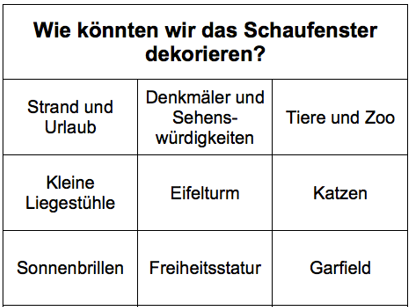
\includegraphics[width=0.5\textwidth]{M635.png}
	\caption{In dieser Abbildung kann erkannt werden, wie Ideen zur Frage: dekoration des Schafensters, entstanden sind}
	%\cite{thirah_vorhangeschloss-schlussel-computer-icons_nodate}
	%\raggedleft
\end{figure}
\newpage
\subsection{Brainstorming}\label{subsec:Brainstorming}

Eine sehr bewährte Variante der Ideenfindung stellt das Brainstorming dar. Hauptsächlich geht es darum, aus möglichst vielen Ideen die besten Ergebnisse herauszufiltern und zu kombinieren. Brainstorming wird am besten in kleineren Gruppen durchgeführt. Wird es in grösseren Gruppen durchgeführt, so entsteht schnell Chaos.

\subsubsection{Vorgehensweise}

\begin{enumerate}
\item In einem ersten Schritt wird ein Moderator erwählt, welcher die Ideen zusammenträgt und diese für alle sichtbar aufschreibt. Alternativ kann auch eine Wandtafel benutzt werden, auf welche jeder seine Ideen aufschreiben kann.
\item In einem zweiten Schritt werden Ideen gesammelt. Dabei kann jeder seine Ideen in einer offenen Runde frei dem Moderator mitteilen oder auf die Tafel schreiben. Dies gewährleistet, dass aus bereits genannten Ideen auch neue Ideen entstehen können. Ein wichtiger Punkt dabei ist, dass keine Idee zu abwegig ist.
\item In einem letzten Schritt werden dann die Ideen sortiert und ausgewertet. Die Teilnehmer sortieren gemeinsam die Ideen und filtern die besten Ideen heraus. Aus diesen Ideen entsteht dann die Zielidee. 

\end{enumerate}
\subsubsection{Vor- und Nachteile}

\begin{tabular}{|l|l|}
	\hline 
	\textbf{Vorteile} & \textbf{Nachteile} \\ 
	\hline 
	Frei Kreativität für jeden & Schwierige Handabung für den Moderator  \\
	\hline 
	Schnelle Ideenfindung & Potential für zu viel input \\ 
	\hline 
	Einbezug aller anwesenden Teilnehmer & Belustigung einzelner bei \flqq abwegigen\frqq  Ideen\\
	\hline
\end{tabular} 


\begin{figure}[h!]
	\centering
	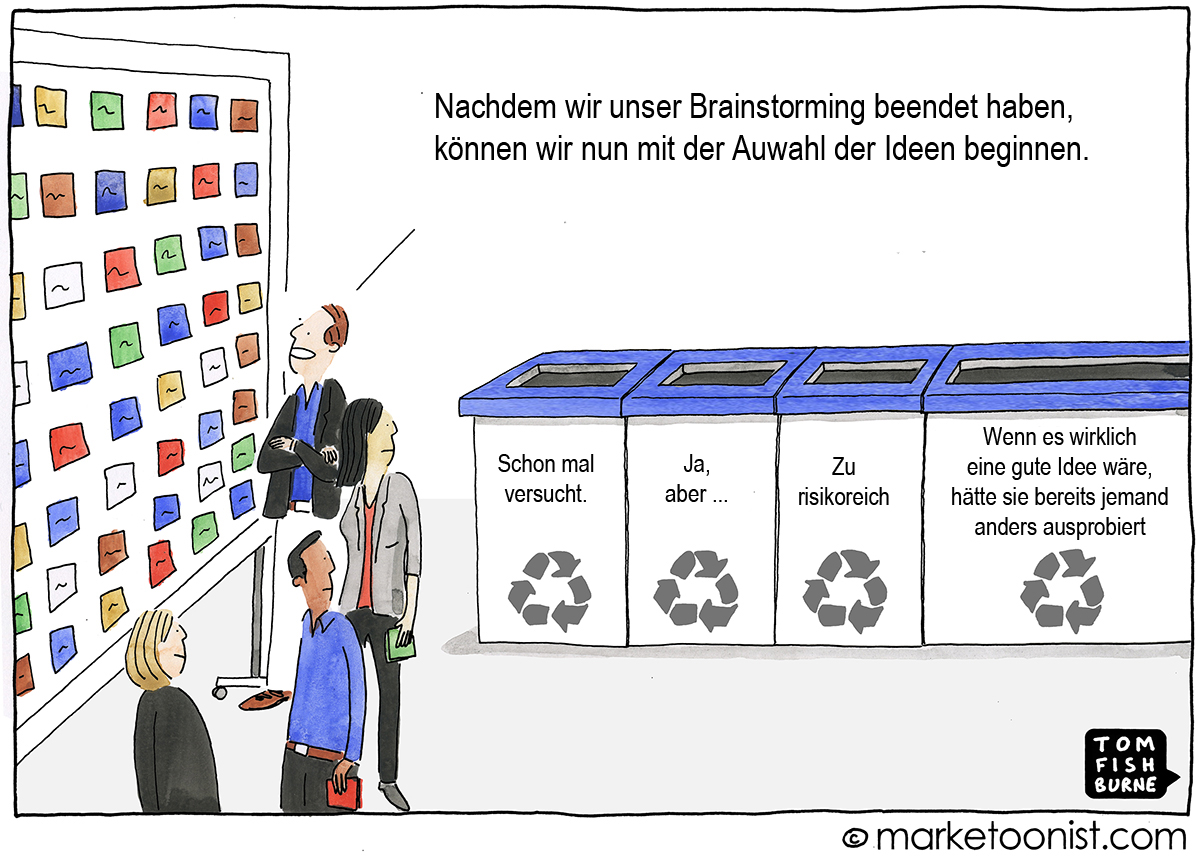
\includegraphics[width=0.8\textwidth]{graphics/Brain}
	\caption{Anschauungsbild Brainstorming}
	\label{fig:Brainstorming}
\end{figure} 




  


%\clearpage
\section{Patentanalyse}\label{sec:Patentanalyse}
\subsection{Beschreibung}\label{subsec:Beschreibung}
Bei dem Patent Planta wird ein freischwingendes Schaltnetzteil beschrieben. Dieses Netzteil enthält folgende Baugruppen: ein Transformator mit einer Leistungswicklung zur Bereitstellung einer Ausgangsspannung, eine Treiberwicklung zur Bereitstellung einer Schaltspannung und eine Reglerwicklung zur Bereitstellung einer Messspannung. Die Ausgangsspannung kann mit Hilfe einer Abschaltspannung von einem Transistor geändert werden. Ein Gleichrichter empfängt die Messspannung und erzeugt eine für die Messspannung repräsentative Steuerspannung. Ein erster Spannungsteiler empfängt die Steuerspannung und schaltet den Schalttransistor ein, wenn die Sperrspannung über einem ersten Schwellwert liegt. Ein zweiter Spannungsteiler empfängt die Steuerspannung und schaltet den Schalttransistor aus, wenn die Sperrspannung unter einem zweiten Schwellwert liegt. Mit diesem Schaltnetzteil wird mit einer Primärsteuerung eine wirksame Spannungsstabilisierung mit einem guten Wirkungsgrad geboten.

\subsection{Schema Patent Palata}\label{subsec:Schema}
\begin{figure}[h!]
	\centering
\rotatebox{-90}{	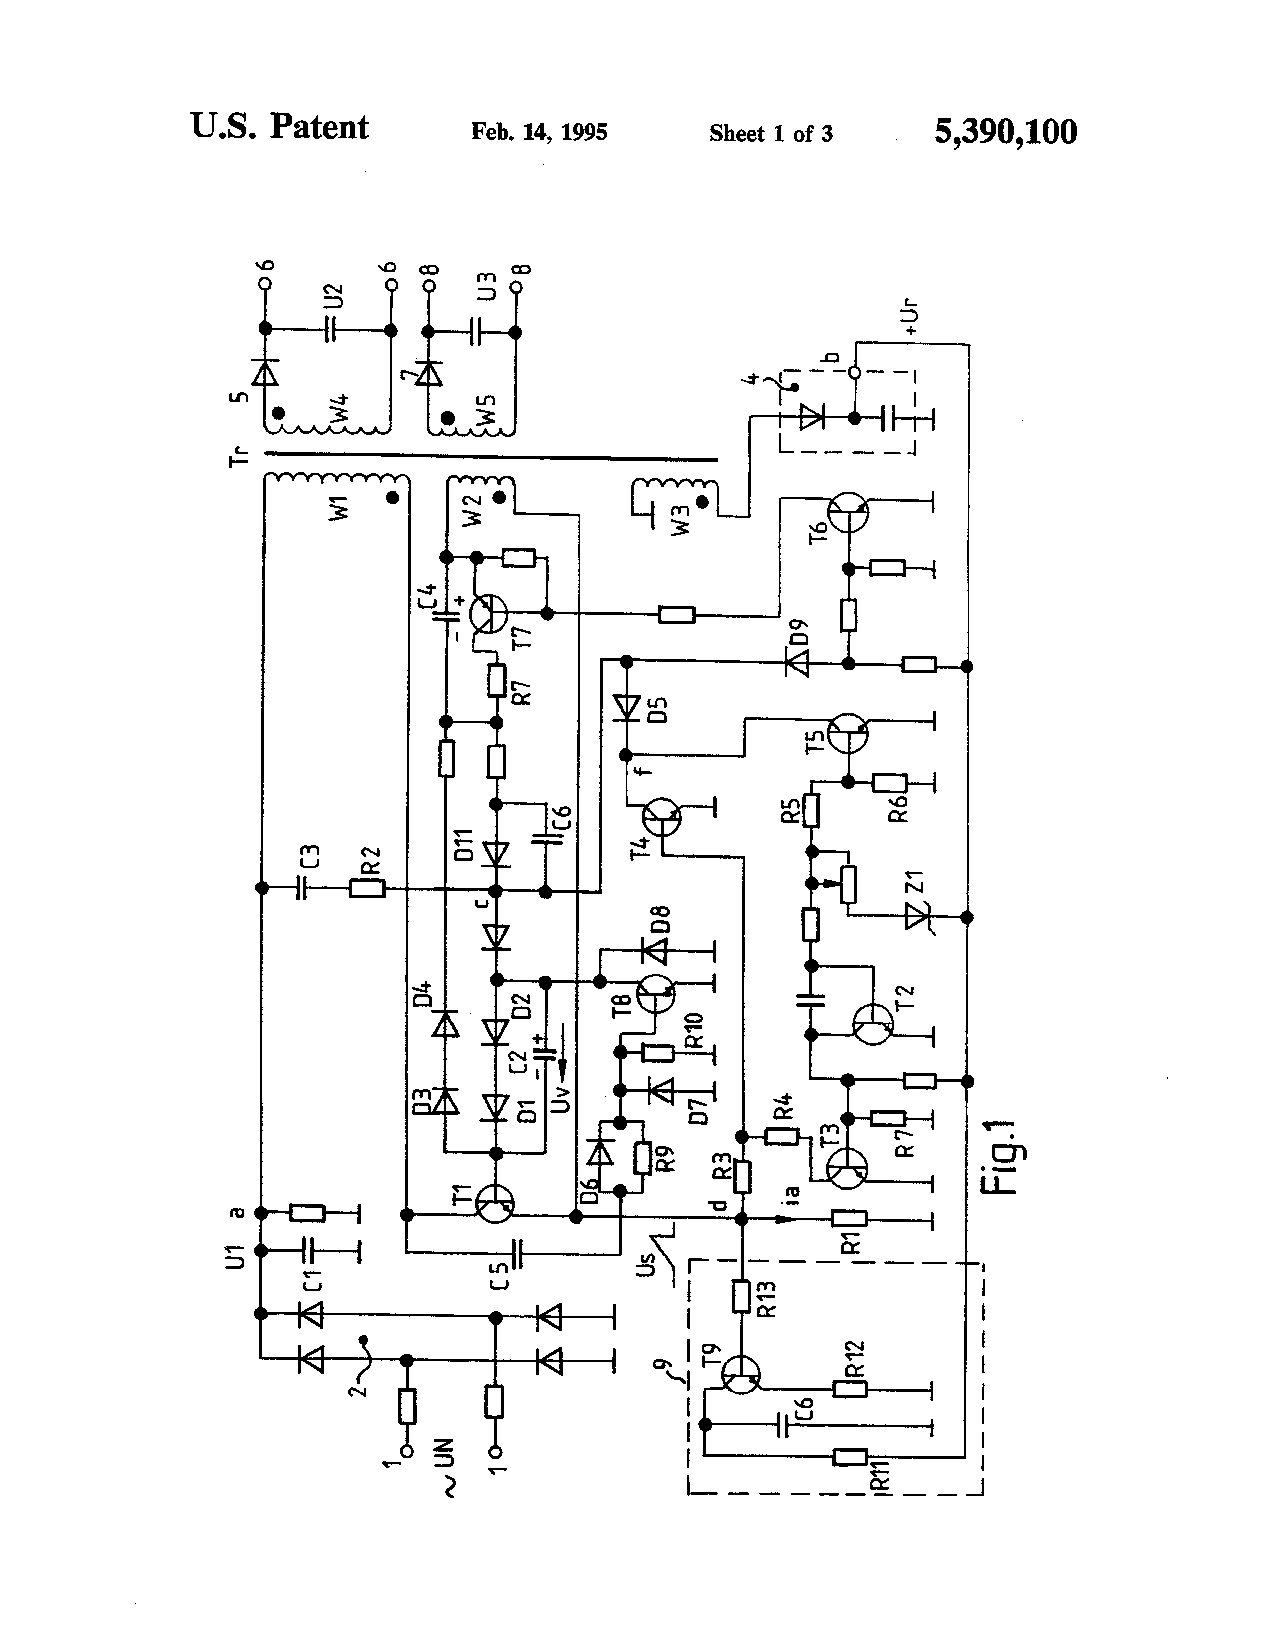
\includegraphics[width=0.7\textwidth]{graphics/Schema}}
	\caption{Schema}
	\label{fig:Schema}
\end{figure} 
\newpage
\subsection{Claim-Chart}\label{sec:Claim-Chart}
In dieser Claim-Chart wird ein Patentverlezugsprozess durchgeführt, nachfolgendes Gerät, welches nach Schema \ref{fig:CCHSchema} und \ref{fig:CCHSchema2} enspricht wurde analysiert.\\
\\

\begin{table}[htbp]
\begin{tabular}{|l|l|l|}
	\hline 
\textbf{US5390100 Planta Claim 1}& &    \\ 
	\hline 
 A freely oscillating switched-mode &A1 & freely oscillating\\
 power supply comprising:	& A2 &switched-mode  \\ 
	\hline 
a transformer having a primary winding,& B1 &primary winding\\
a secondary winding for providing &B2,B3 &secondary winding\\ 
an output voltage, and a regulating& B4&regulating winding\\
winding for providing a& & \\
measuring voltage; & &	 \\
	\hline 
a switching transistor, having a cutoff& C1 & switching transistor \\
voltage and being coupled to said  &C2  &coupled to said primary winding \\
primary winding for controlling & & \\
current therein;	&  &  \\ 
	\hline 
means for generating a control voltage& D1 & means for generating a control voltage\\
coupled to said measuring voltage;	&  & \\ 
	\hline 
first feedback means for varying said & E1 &first feedback\\
cutoff voltage responsive to said  &  &\\
control voltage when said control & &\\
voltage exceeds a first threshold value;  & &\\ 
	\hline 
second feedback means responsive to& F1&secound feedback\\
said control voltage for initiating  &  &\\
burst mode operation of said switching& & \\
transistor when said control voltage & &\\
exceeds a second threshold value.	&  &  \\ 
	\hline 
\end{tabular}
\caption{Claim Chart Tabelle}
\label{tab:Claim} 
\end{table}





\begin{figure}[h!]
	\centering
	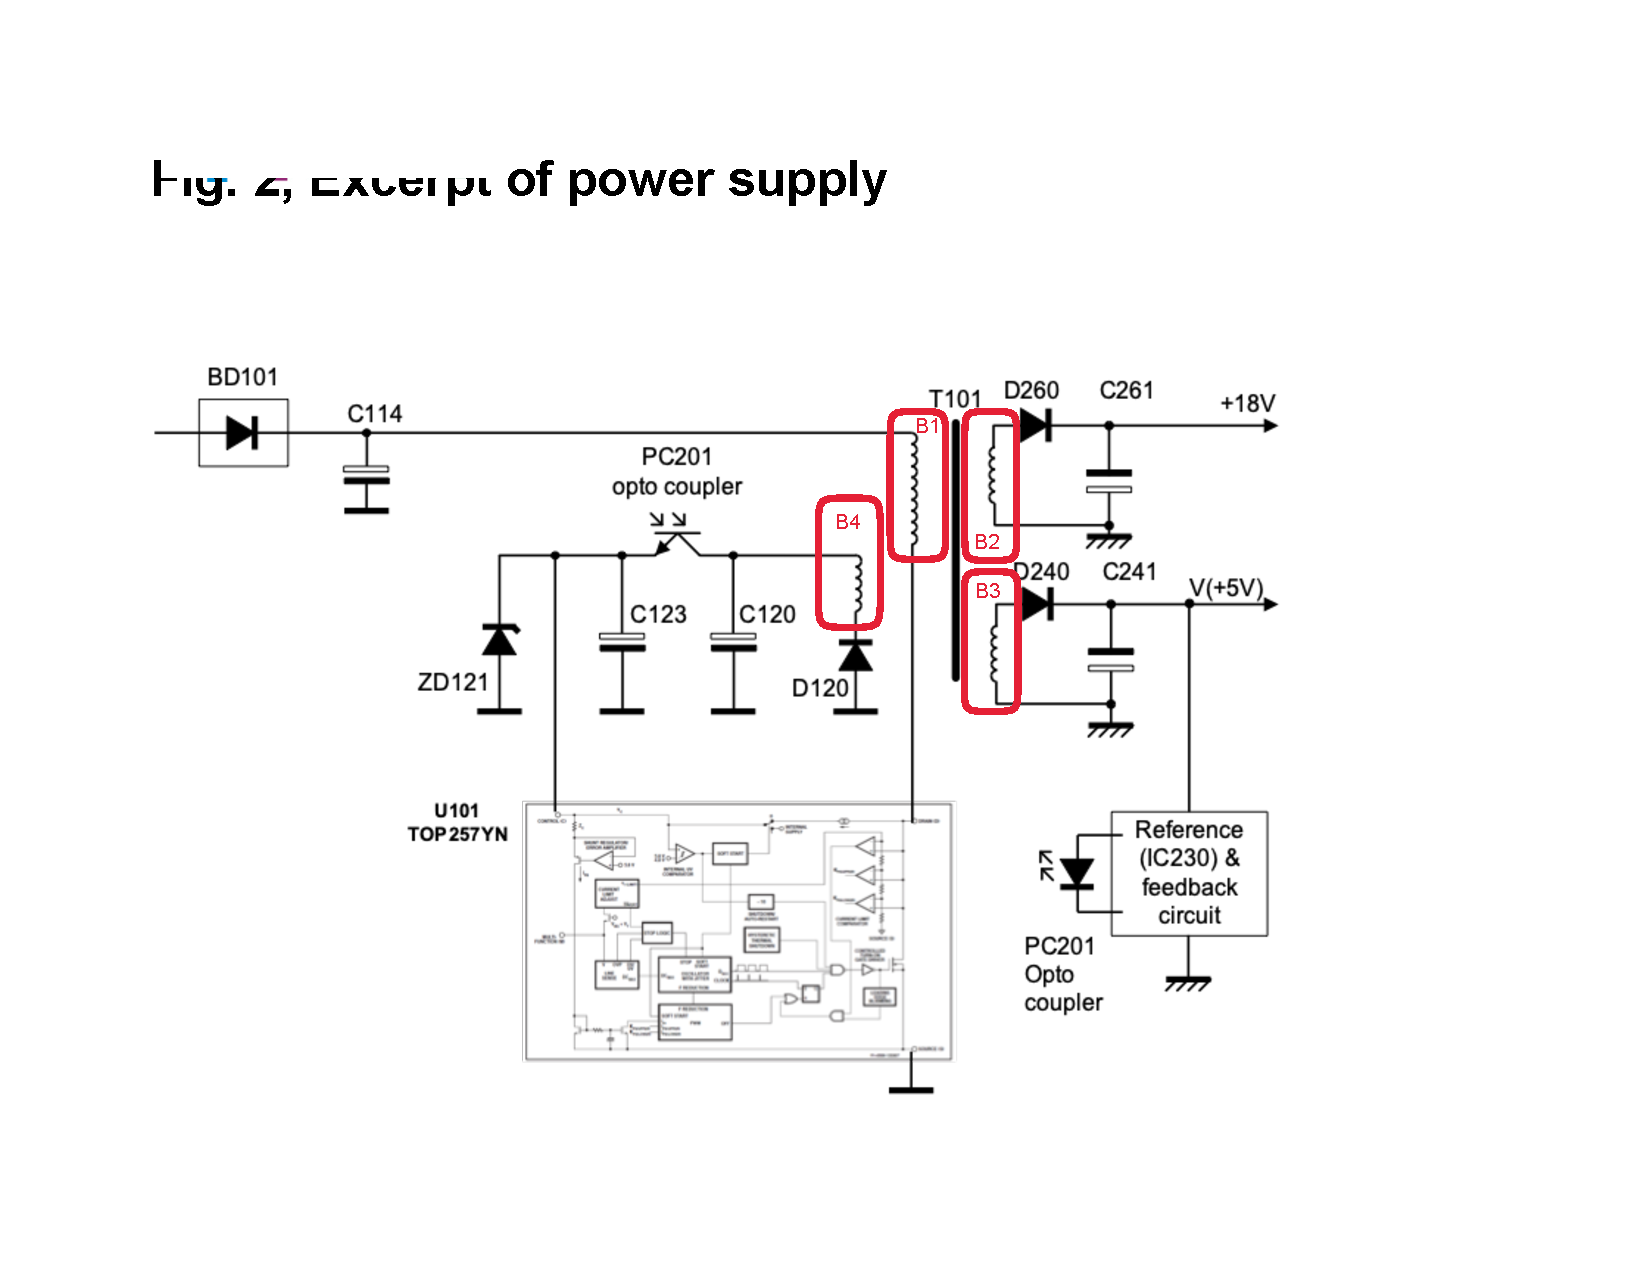
\includegraphics[trim = 20mm 20mm 50mm 50mm, clip, width=1\textwidth]{graphics/SchemaClaim}
	\caption{Claim Chart Schema Schaltnetzteil}
	\label{fig:CCHSchema}
\end{figure} 
\newpage

\begin{figure}[h!]
	\centering
	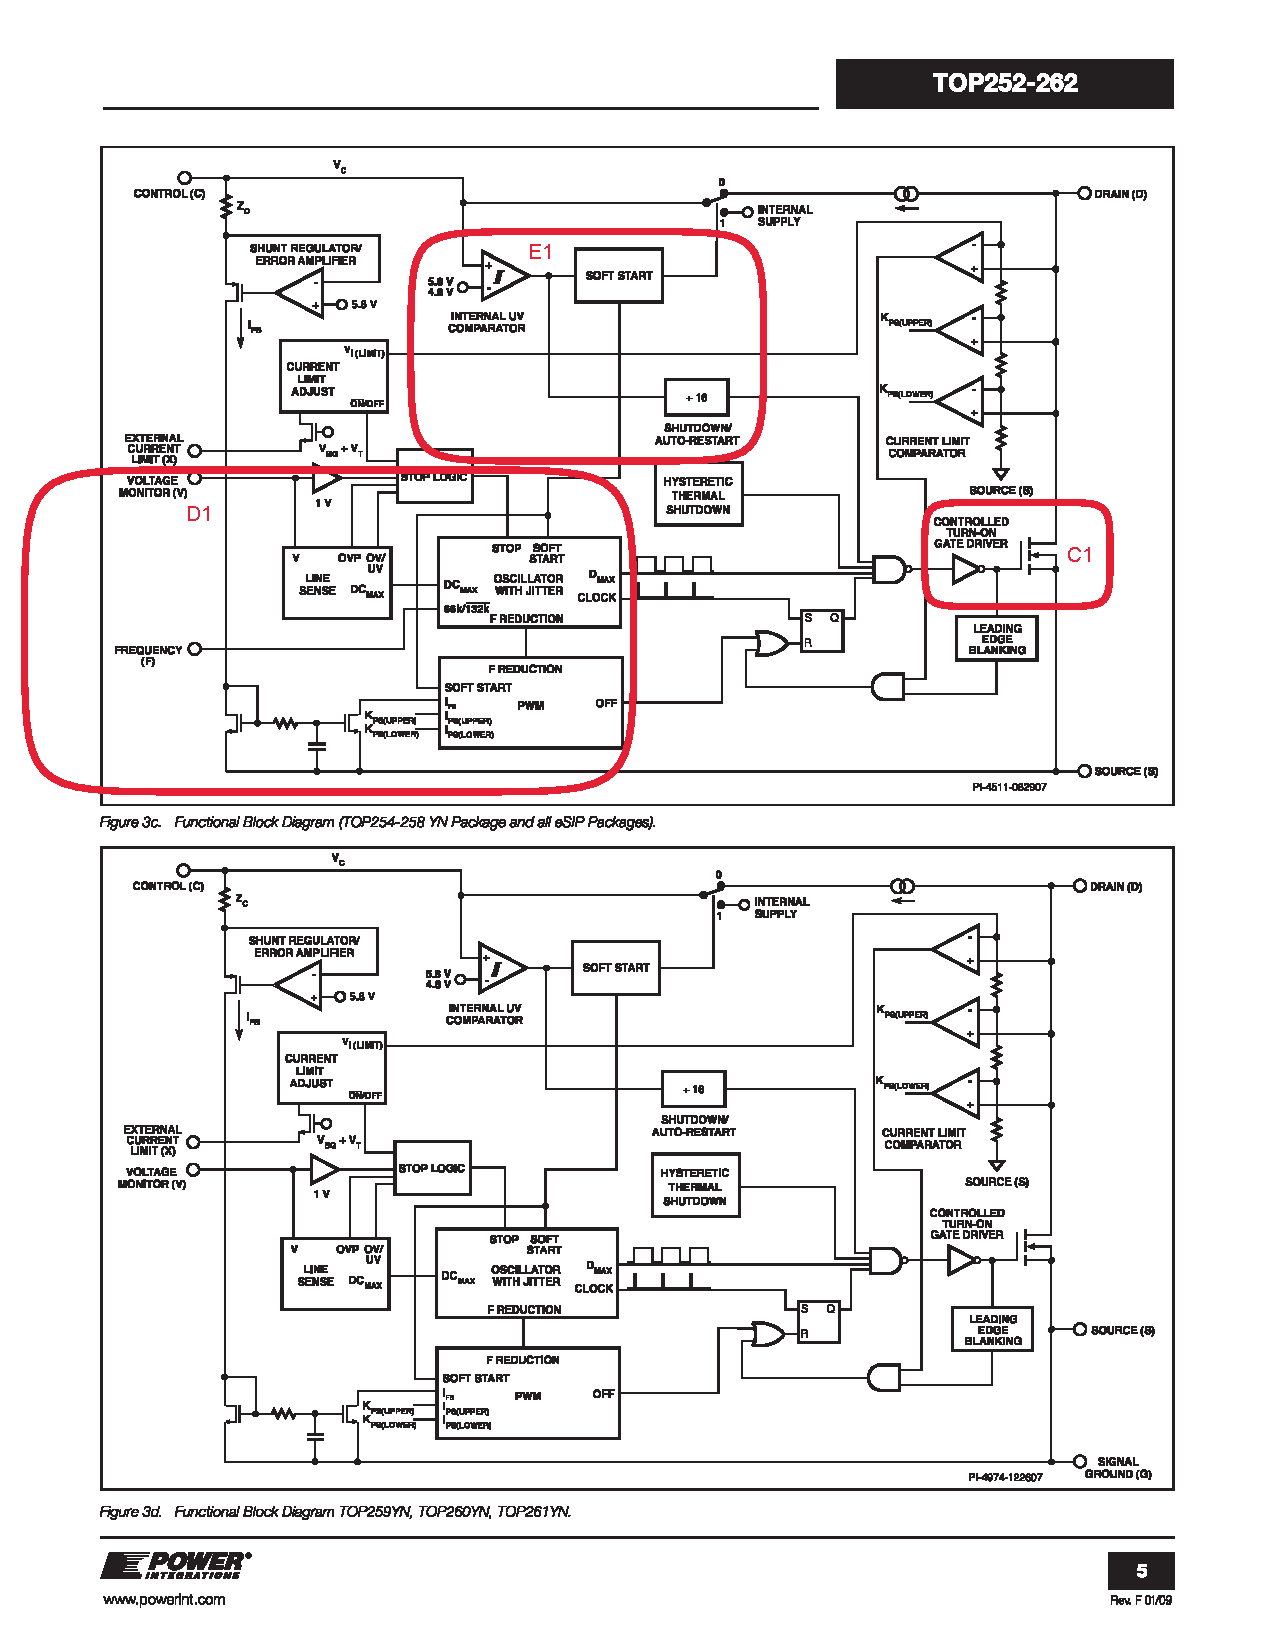
\includegraphics[trim = 1mm 142mm 1mm 20mm, clip, width=1\textwidth]{graphics/SchemaClaim2}
	\caption{Claim Chart Schema TOP257YN}
	\label{fig:CCHSchema2}
\end{figure} 

\subsection{Messungen}\label{sec:Messungen}

In der Messtabelle \ref{fig:Schalttransistor} ist ersichtlich, dass der Schalttransistor bei unterschiedlichen Belastungen anders agiert. Somit ist die Einschaltdauer (On-time) ohne Belastung bei 1.8us, wobei sie wiederum bei einer Belastung von 50W bei 5.1us liegt. Auch ersichtlich ist dabei die jeweilige Messspannung (measuring voltage) gemäss \ref{tab:Claim}.

\begin{figure}[h!]
	\centering
	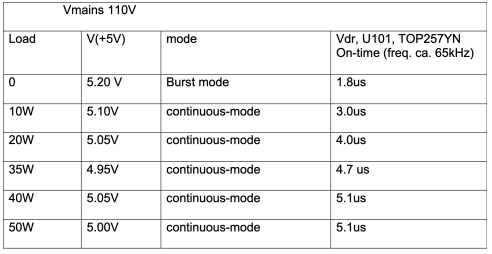
\includegraphics[width=0.8\textwidth]{graphics/Messtabelle}
	\caption{Messtabelle der Einschaltzeiten des Schalttransistors}
	\label{fig:Schalttransistor}
\end{figure} 

In Abbildung \ref{fig:cutoff} ist das Schaltverhalten des Schalttransistors (cutoff voltage) in Abhängigkeit der Kontrollspannung (control voltage) gemäss Tabelle \ref{tab:Claim} zu sehen. \\

\begin{figure}[h!]
	\centering
	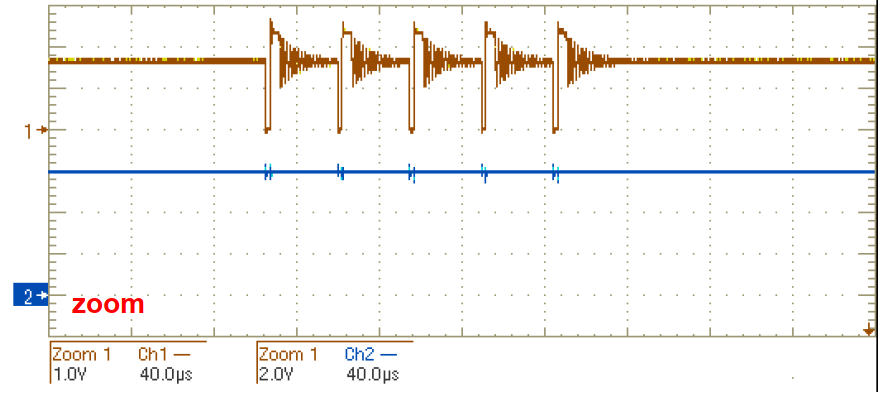
\includegraphics[width=0.8\textwidth]{graphics/cutoff}
	\caption{Messung der cutoff voltage, in Abhängigkeit der control voltage}
	\label{fig:cutoff}
\end{figure} 

Mit diesen Messungen ist es ersichtlich, dass die Ausgangsspannung (output voltage) von 18V gemäss \ref{fig:CCHSchema} über eine Messpannung (measuring voltage)leistungsangepasst ist.

\newpage



 
 
 

%\clearpage
\section{Fazit}\label{sec:Fazit}
Mit dieser Arbeit konnte erkannt werden, dass verschiedene Patentierte Erfindungen von Palata, in dem zu analysierendem Gerät angewendet wurden. Das Patent Palata wurde verletzt und ein Patentanspruch kann abgehandelt werden. Wird in den Rechtsgrundlagen recherchiert kann zwischen unmittelbarer und mittelbarer Patentverletzung unterschieden werden. Bei unmittelbarer Patentverletzung ist alleine der Patentinhaber befugt, die patentierte Erfindung zu benutzen, was gesetzlich im Patentgesetz (PatG) verfasst ist. Bei der mittelbaren Patentverletzung erstreckt sich der Geltungsbereich der patentierten Erfindung noch weiter als bei den unmittelbaren Benutzungshandhabungen, es untersagt Dritten auch die Benutzung derjenige Mittel, die sich auf ein wesentliches Element der Erfindung beziehen.
\pagebreak


%\clearpage
%%---BIBLIOGRAPHY------------------------------------------------------------------------


{\sloppypar
%\printbibliography[heading=bibnumbered ]
\label{sec:lit}
\selectlanguage{ngerman}				%ngerman or english
\printbibliography
}

%\pagebreak

%\input{sections/8_0_Ehrlichkeitserklaerung}
%\pagebreak
%%---APPENDIX----------------------------------------------------------------------------
%\appendix
%%\begin{appendix} %Anhang


%Anhang A
%\includepdf[pages={1},nup=1x1,landscape=false,scale=0.90, pagecommand = \section*{\LARGE{Anhang:}}
%\addcontentsline{toc}{section}{Anhang}
%\section{Auftrag des Arbeitgebers}
%\label{app:Lastenheft}, offset =0mm -22mm ]{appendix/Lastenheft.pdf}\newpage
%Bei mehrseitigen Dokumenten die folgenden Seiten ohne Überschrift:
%\includepdf[pages={2},nup=1x1,landscape=false,scale=0.90,offset=6 -30,pagecommand={\thispagestyle{myheadings}}]{appendix/Lastenheft.pdf} 
%\newpage


%Anhang B: Bestimmung der Ersatzelemente der ASM
%\input{sections/ASM_Laborjournal}


%Anhang C: Messungen für ADC-Verifikation
\clearpage
\section{Messungen Zeitverzögerung Modulator}\label{app:Messungen_Delay Modulator}



\begin{figure}[H]
	\centering
	\includegraphics[width=0.85\linewidth]{appendix/Delay_modulator.png}
	\caption{Messung der Zeitverzögerung zwischen Modulatoreingang und modulierter Spannung an der ASM}
	\label{fig:app_delay}
\end{figure}


%Beispiel für A3 Seite einfügen:

%Anhang B
%A3
%\eject\pdfpagewidth=420mm \pdfpageheight=297mm
%A3


%Anhang B: Schema Layout
%\includepdf[pages={1},nup=1x1,landscape=false,scale=1.7,offset=300 -50,pagecommand={\section{Schema BMS-Slave}\label{app: Schema_Layout}\thispagestyle{myheadings}}]{appendix/Schema_Layout_.pdf} \newpage

%A4
%\eject\pdfpagewidth=210mm \pdfpageheight=297mm
%A4


%Beispiel Anhang C: (PDF)



%Anhang C: Dimensionierung passives Balancing
%\includepdf[pages={1},nup=1x1,landscape=false,scale=0.90,offset=10 -40,pagecommand={\section{Dimensionierung passives Balancing}\label{app: Dimensionierung_Balancing}\thispagestyle{myheadings}}]{appendix/Dimensionierung_Balancing.pdf} 
%\newpage


%\end{appendix}


%%---NOTES for DEBUG---------------------------------------------------------------------
%\ifdraft{%Do this only if mode=draft
%\usepackage{todonotes})
%\newpage
%\listoftodos[\section{Todo-Notes}]
%\clearpage
%}
%

\end{document}
